\documentclass[border=10pt]{standalone}

\usepackage{tikz}
\usepackage{tikzsymbols}
\usetikzlibrary{calc,patterns,shapes.geometric}

\def\centerarc[#1](#2)(#3:#4:#5){\draw[#1] ($(#2)+({#5*cos(#3)},{#5*sin(#3)})$) arc (#3:#4:#5);}

\begin{document}
	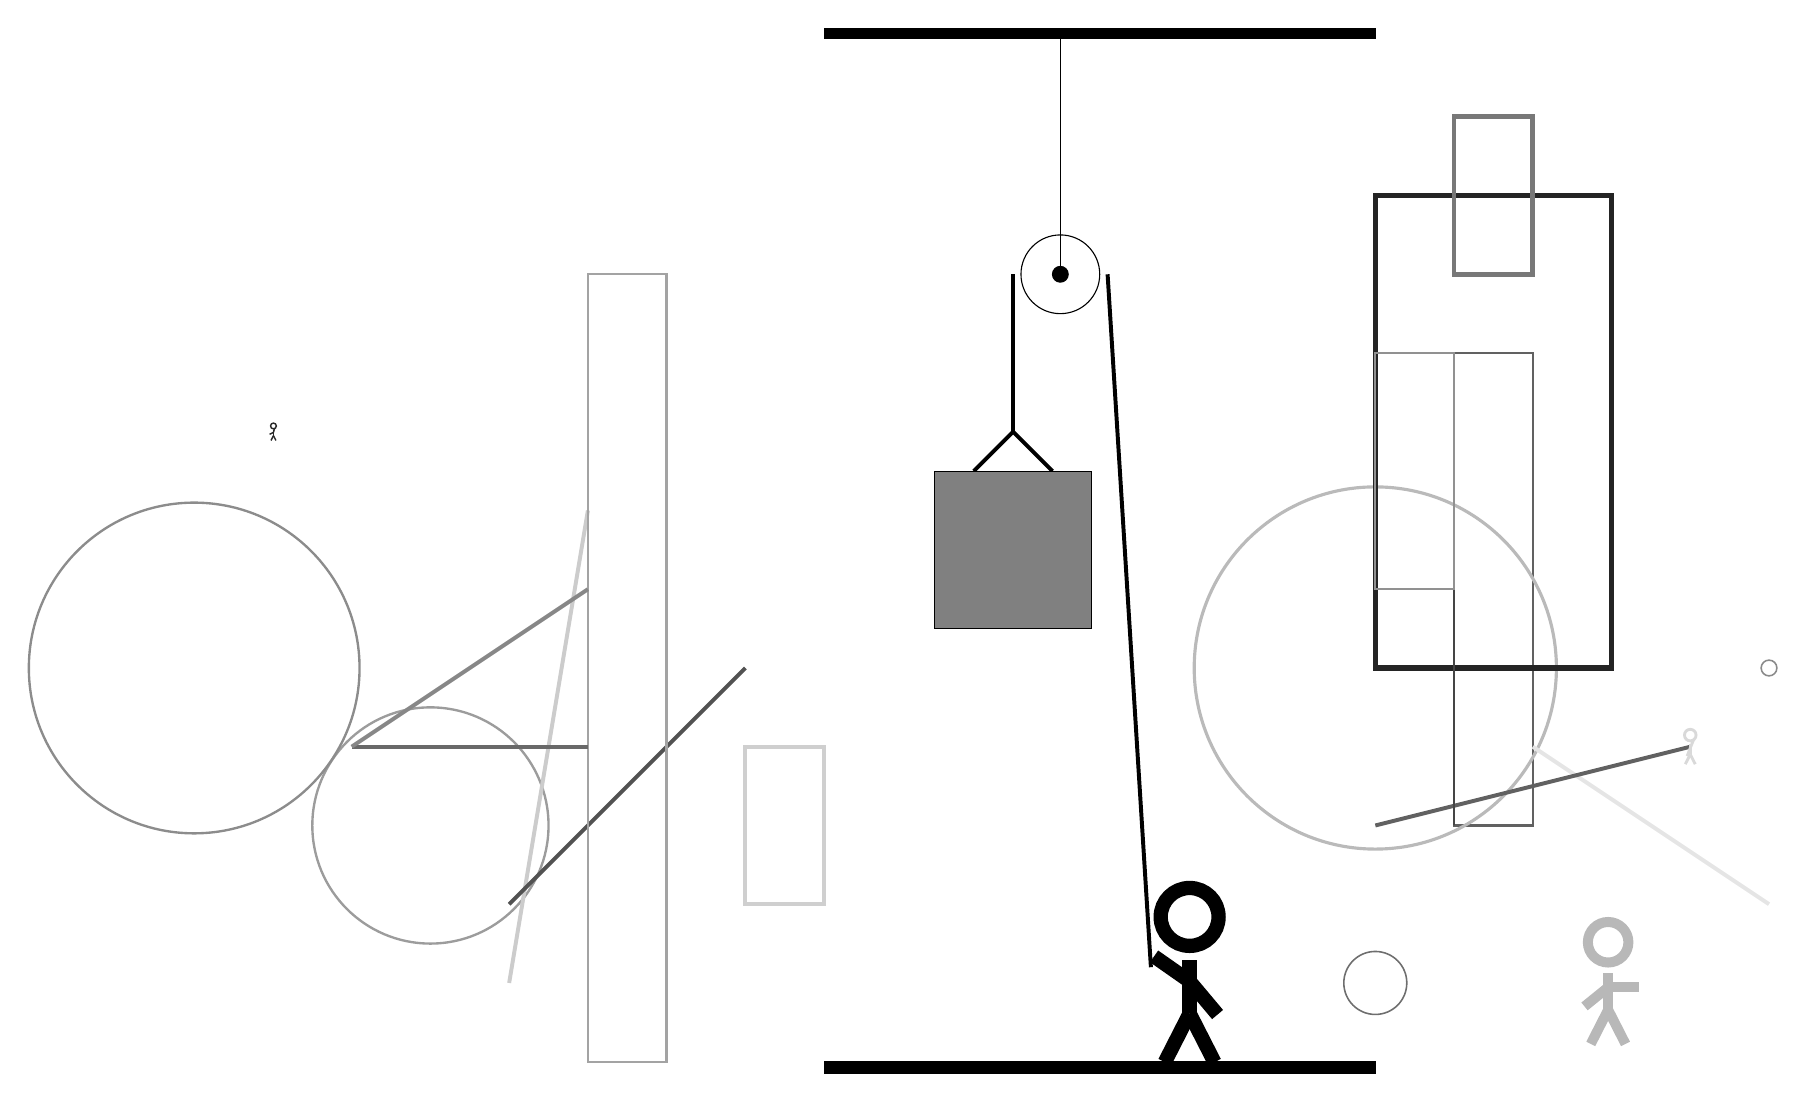
\begin{tikzpicture}
		%%%%% START %%%%%
		
		\draw[fill=black] (-2, 10) rectangle (5, 10.125);
		
		\draw (1, 7) circle (0.5);
		\draw[fill=black] (1, 7) circle (0.1);
		\draw (1, 10) -- (1, 7);
		
		\draw[line width=0.5mm] (-0.1, 4.5) -- (0.4, 5.0) -- (0.9, 4.5);
		\draw[fill=black!50] (-0.6, 4.5) rectangle (1.4, 2.5);
		
		\draw[line width=0.5mm] (0.4, 7) -- (0.4, 5.0);
		\centerarc[line width=0.5mm](1, 7)(0:180:0.6);
		\draw[line width=0.5mm](1.6, 7) -- (2.15, -1.8);
		
		\node at (2.6, -1.9) {\Strichmaxerl[10][-35][-50]};
		
		\draw[line width=0.3mm, color=black!62] (6, 0) rectangle (7, 6);
		
		\draw[line width=0.2mm, color=black!22] (6, 6) rectangle (6, 1);
		\draw [line width=0.4mm, color=black!27](5, 2) circle (2.3);
		\draw[line width=0.7mm, color=black!86] (5, 8) rectangle (8, 2);
		\draw[line width=0.5mm, color=black!10](7, 1) -- (10, -1);
		
		\draw [line width=0.3mm, color=black!39](-7, 0) circle (1.5);
		\draw [line width=0.2mm, color=black!46](10, 2) circle (0.1);
		
		\draw[line width=0.6mm, color=black!53] (6, 9) rectangle (7, 7);
		\draw [line width=0.2mm, color=black!57](5, -2) circle (0.4);
		\draw[line width=0.5mm, color=black!20](-5, 4) -- (-6, -2);
		\draw[line width=0.5mm, color=black!68](-3, 2) -- (-6, -1);
		\draw[line width=0.5mm, color=black!62](5, 0) -- (9, 1);
		\node[line width=0.5mm, color=black!15] at (9, 1) {\Strichmaxerl[2][69][68]};
		\draw[line width=0.3mm, color=black!73] (6, 0) rectangle (6, 4);
		\draw[line width=0.3mm, color=black!43] (5, 3) rectangle (6, 6);
		\draw [line width=0.3mm, color=black!45](-10, 2) circle (2.1);
		
		\node[line width=0.5mm, color=black!84] at (-9, 5) {\Strichmaxerl[1][26][74]};
		
		\draw[line width=0.3mm, color=black!36] (-4, 7) rectangle (-5, -3);
		\node[line width=0.7mm, color=black!28] at (8, -2) {\Strichmaxerl[7][39][0]};
		\draw[line width=0.5mm, color=black!59](-5, 1) -- (-8, 1);
		\draw[line width=0.5mm, color=black!47](-5, 3) -- (-8, 1);
		\draw[line width=0.5mm, color=black!19] (-2, -1) rectangle (-3, 1);
		
		
		\draw[fill=black] (-2, -3) rectangle (5, -3.15);
		
		%%%%% END %%%%%
	\end{tikzpicture}
\end{document}